\documentclass[../../main.tex]{subfiles}
\usepackage{graphicx}
\graphicspath{{./figure/}}
\DeclareGraphicsExtensions{.png}
\begin{document}

\section{补图、偶图}
\begin{enumerate}
    \item $G$ 不是连通图,则存在 $m \ge 2$ 个支 $G_1,G_2,\cdots G_m$,任取两点 $u,v$,若 $u,v$ 在同一个支 $G_i$ 中,则在补图 $G^{c}$ 中存在 $ux,vx$ 两条边使其连通,其中 $x$ 是另外一支的一个点。若 $u,v$ 在不同支则 $u,v$ 有边连通。
    \item 待补充
    \item 显然每个自补图所对应的完全图边数都是偶数,即 $\frac{p(p-1)}{2}$ 是偶数,即 $p$ 为 $4n$ 或 $4n+1$
    \item 没有三角形我们考虑构造一个偶图,将点划分为 $U,V$ 两个集合 $|U|=|V|=n$,连边为 $u_1v_1,u_2v_2,\cdots u_nv_n$,$u_1v_2,u_2v_3,\cdots u_{n-1}v_n$,$u_2v_1,u_3v_2,\cdots u_nv_{n-1}$ 与 $u_1v_n,u_nv_1$ 
    \begin{figure}[htpbp]
        \centering
        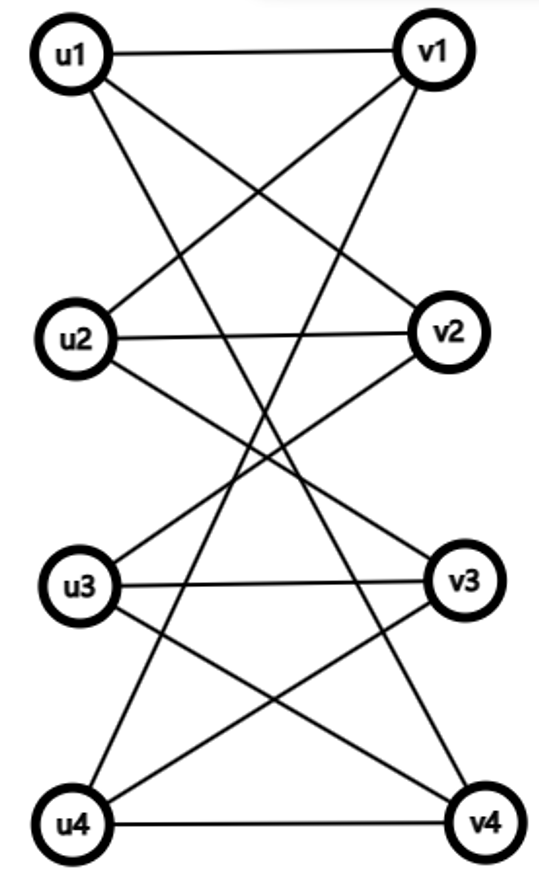
\includegraphics[width=3cm]{graph01}%
        \caption{示例}
    \end{figure}
    \item 因为 $A$ 是0点,$B$ 是1点,从A到B一定走了奇数步,但是不重不漏的走完整个棋盘需要偶数步,所以不可能
    \item 下面对 $p$ 是偶数证明,$p$ 是奇数应该也差不多。先证明没有度数大于 $\frac{p}{2}$ 的点,若存在度数最大的点 $v$ 有 $d(v) > \frac{p}{2}$,则他所连的 $d(v)$ 个点中每个点度数都小于 $n-d(v)$,则 $2q \le d(v)+(d(v)-1)(p-d(v))+d(v)(p-d(v)-1)=(p-d(v))(2d(v)-1)$ 可知 $(p-d(v))(2d(v)-1)$ 是小于 $\frac{p^2}{2}$ 的,所以最大度数小于等于 $\frac{p}{2}$,又$p\times \frac{p}{2}=\frac{p^2}{2}$,所以该图为 $\frac{p}{2}$ 正则图。且该图没有三角形,则由 6.3 节习题10可证得结论
    \item 建议搜索图兰定理,该定理有很多证明方法
    \item 对格子黑白染色,每个骨牌会覆盖一个黑格子和一个白格子,删去两个白格子后黑格子和白格子数量不等,无法用骨牌覆盖
    \item 反证,若 $G^c$ 中有 $u,v$ 使得 $d(u,v) \ge 3$,则 $\forall x \in G$ $ux,vx$ 都不在 $G^{c}$ 中,则 $ux,vx$ 在 $G$ 中,则对于 $x,y \in G$,有路 $xuvy$ 长度为 $3$,与 $G$ 直径大于 $3$ 矛盾。
    \item \begin{enumerate}
        \item 显然每个顶点有 $k$ 条边,边数为 $k2^{k-1}$
        \item 这是自然的
        \item 使得,假设存在一个奇数长度的圈 $C$,设其长度为 $2n+1$,则某个顶点 $(a_1,a_2,\cdots,a_k)$ 改变了奇数次变回自身,这是不可能的。所以这是一个偶图
    \end{enumerate}
\end{enumerate}
\end{document}